\documentclass{sciposter}
\usepackage{lipsum}
\usepackage{epsfig}
\usepackage{amsmath}
\usepackage{amssymb}
\usepackage{multicol}
\usepackage{graphicx,url}
\usepackage[portuges, brazil]{babel}
\usepackage[utf8]{inputenc}
%\usepackage{fancybullets}
\newtheorem{Def}{Definition}


\title{Classic Methods on \\Color Based Ball Tracking}
%Título do projeto

\author{Breno Leite\\Guilherme Leite}
%nome dos autores

\institute
{Introduction to Computer Vision\\
Instituto de Computa\c{c}\~ao -- UNICAMP}
%Nome e endereço da Instituição

\email{{brenolleite, guilherme.vieira.leite},{(@gmail.com})}
% Onde você coloca os emails dos integrantes


%\date is unused by the current \maketitle

\rightlogo[1]{ic-logo}
\leftlogo[1]{unicamp-logo}
% Exibe os logos (direita e esquerda)
% Procure usar arquivos png ou jpg, e de preferencia mantenha na mesma pasta do .tex
%%%%%%%%%%%%%%%%%%%%%%%%%%%%%%%%%%%%%%%%%%%%%%%%%%%%%%%%%%%%%%%%%%%%%%%%%%%%%%%%
%%% Begin of Document



\begin{document}
%define conference poster is presented at (appears as footer)

%\LEFTSIDEfootlogo
% Uncomment to put footer logo on left side, and
% conference name on right side of footer

% Some examples of caption control (remove % to check result)

%\renewcommand{\algorithmname}{Algoritme} % for Dutch

%\renewcommand{\mastercapstartstyle}[1]{\textit{\textbf{#1}}}
%\renewcommand{\algcapstartstyle}[1]{\textsc{\textbf{#1}}}
%\renewcommand{\algcapbodystyle}{\bfseries}
%\renewcommand{\thealgorithm}{\Roman{algorithm}}

\maketitle

%%% Begin of Multicols-Enviroment
\begin{multicols}{3}

%%% Abstract

%%% Introduction
\section{Motivation}

Ball tracking is a classical problem present in a diverse range of applications. Nowadays it is used in sports events to automatically track the focus of the action and game score, it is also widely used in robotics, specially in robocup's soccer competitions.

\section{Methodology}

In all the experiments the tracking was performed in a controlled environment. Our objective is to show the performance of the classical methods applied in this project, like color detection, hough circle transform, motion flow, and kalman filter .

\bigbreak

The following scenarios were used to analyze the overall performance of the proposal.

\begin{itemize}

\item \textbf{Controlled environment} - Under artificial light, using the same objects on a clean bland background, in which simple trajectories are performed.
\item \textbf{Real World environment} - Noisy and moving background, under different light sources, in which unpredictable trajectories are performed.  

\end{itemize}

\section{Experiments}

We approached all the scenarios listed above in a incremental complexity manner.

\bigbreak
\textbf{Single colored ball detection}:

\begin{figure}[!h]
	\centering
			\setlength{\fboxsep}{1pt}
			\setlength{\fboxrule}{1pt}
			\fbox{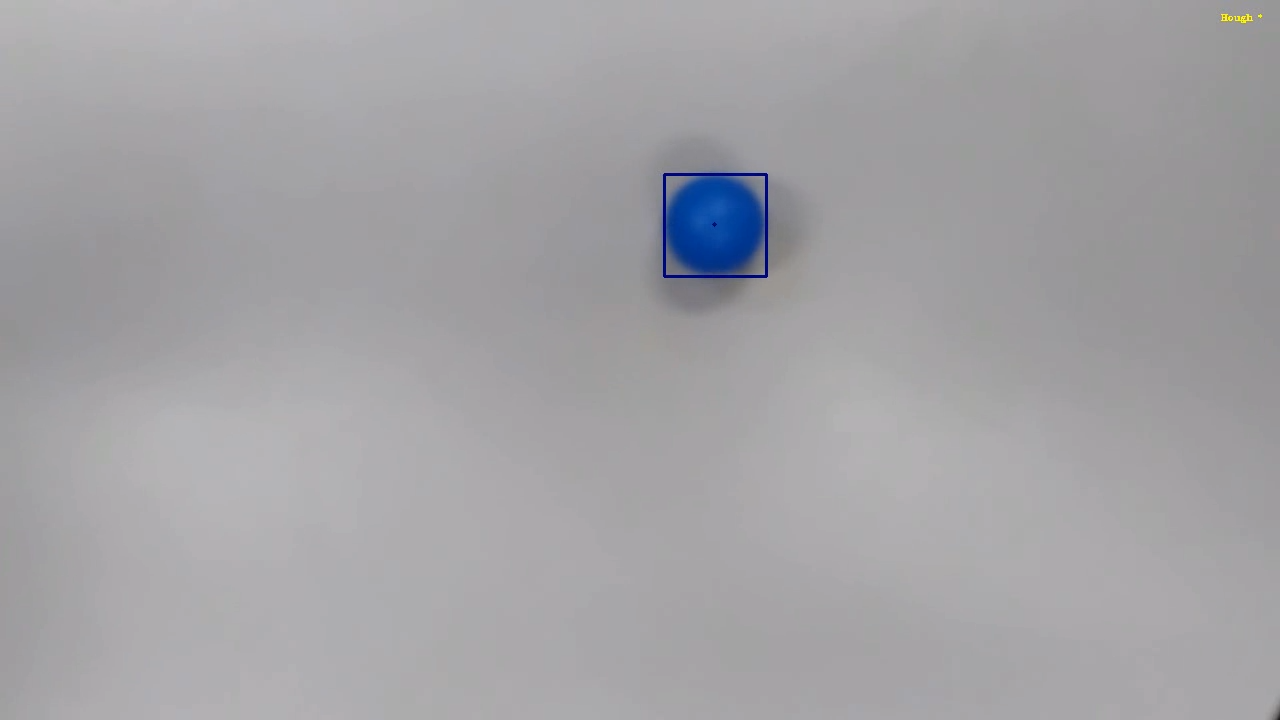
\includegraphics[scale=0.5]{images/single_color}}
	\caption{Detection of a colored ball.}
	\label{fig:single_color}
\end{figure}

\textbf{Different colored balls detection}:

\begin{figure}[!h]
	\centering
			\setlength{\fboxsep}{1pt}
			\setlength{\fboxrule}{1pt}
			\fbox{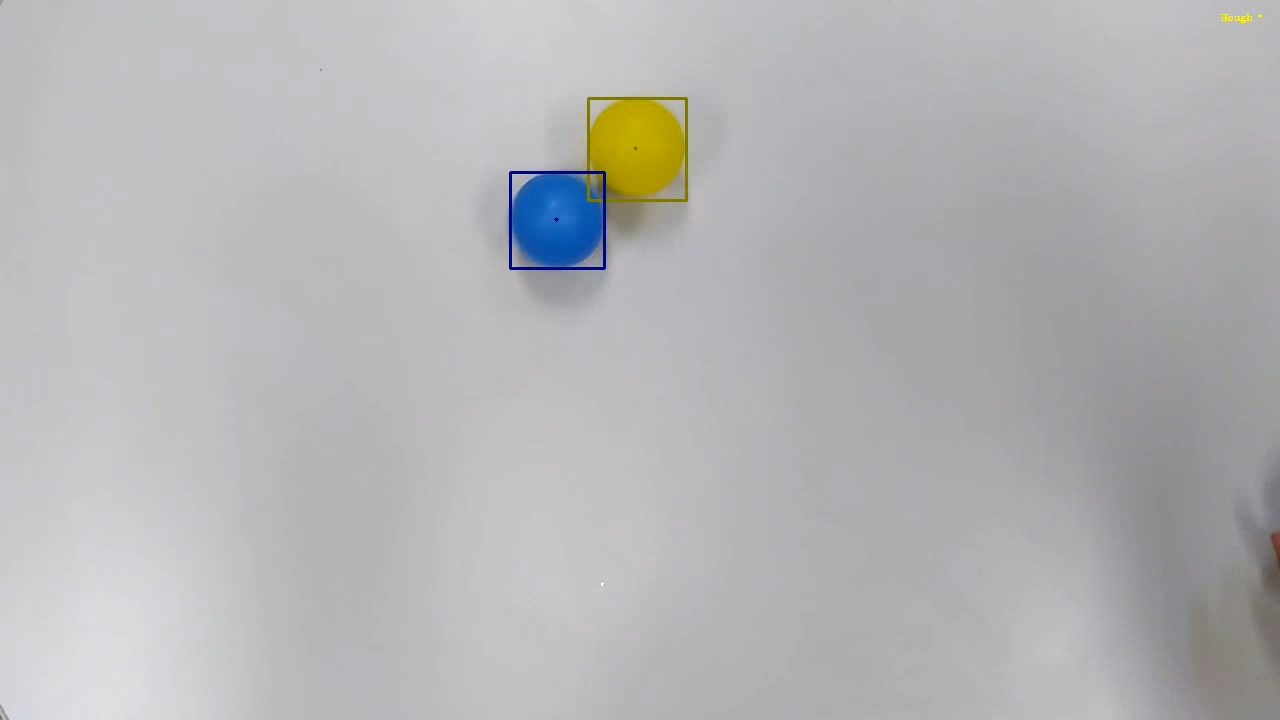
\includegraphics[scale=0.5]{images/diff_color}}
	\caption{Detection of two different colored balls.}
	\label{fig:diff_color}
\end{figure}

\textbf{Same colored balls detection}:

\begin{figure}[!h]
	\centering
			\setlength{\fboxsep}{1pt}
			\setlength{\fboxrule}{1pt}
			\fbox{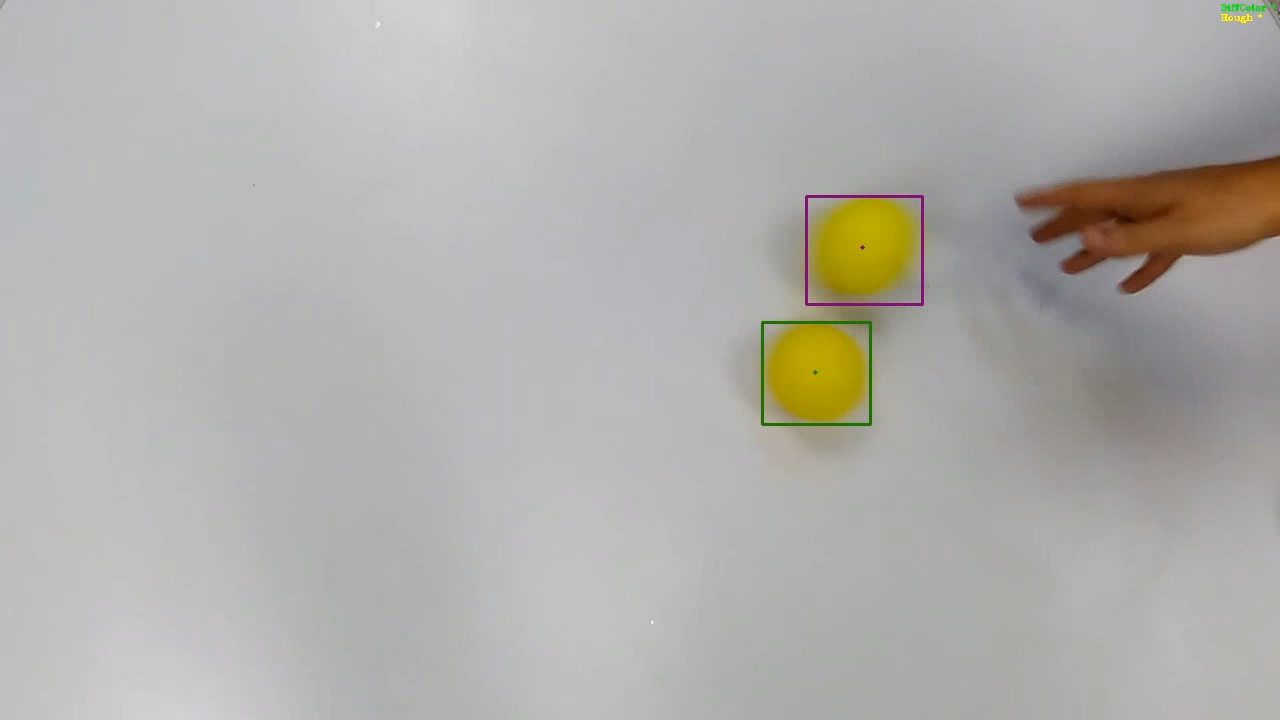
\includegraphics[scale=0.5]{images/same_color}}
	\caption{Detection of same color balls as unique subjects.}
	\label{fig:same_color}
\end{figure}

\textbf{Object detection without Hough Transform}:

\begin{figure}[!h]
	\centering
			\setlength{\fboxsep}{1pt}
			\setlength{\fboxrule}{1pt}
			\fbox{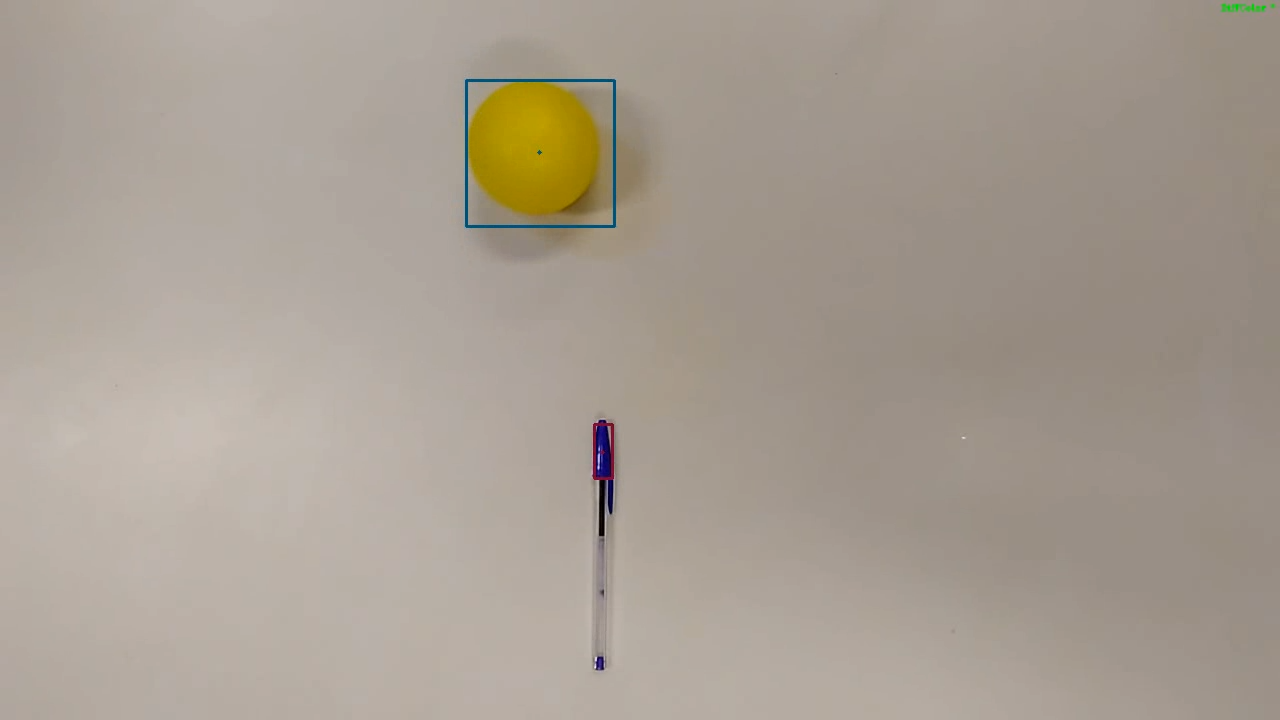
\includegraphics[scale=0.5]{images/not_hough}}
	\caption{Detector mistakenly detecting the pen as a ball.}
	\label{fig:not_hough}
\end{figure}

\textbf{Object detection with Hough  Transform}:

\begin{figure}[!h]
	\centering
			\setlength{\fboxsep}{1pt}
			\setlength{\fboxrule}{1pt}
			\fbox{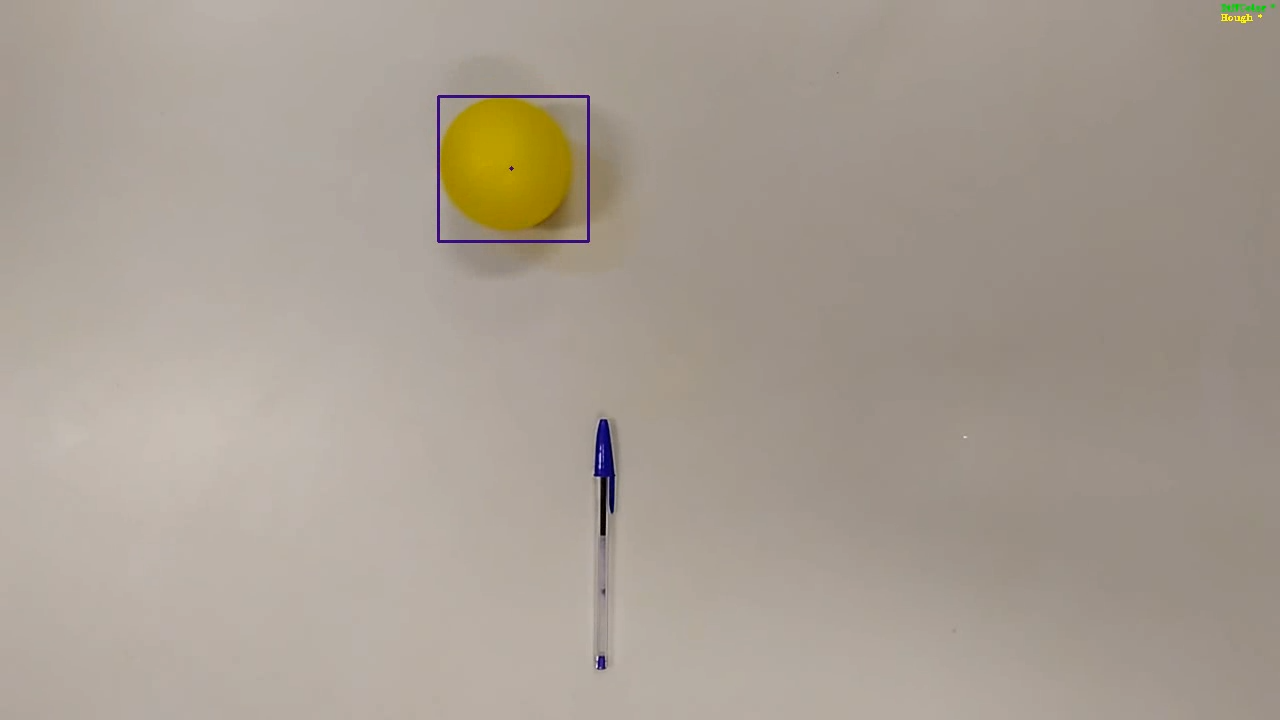
\includegraphics[scale=0.5]{images/yes_hough}}
	\caption{Detector ignoring the pen.}
	\label{fig:yes_hough}
\end{figure}

\textbf{Lucas Kanade Motion Flow}:

\begin{figure}[!h]
	\centering
			\setlength{\fboxsep}{1pt}
			\setlength{\fboxrule}{1pt}
			\fbox{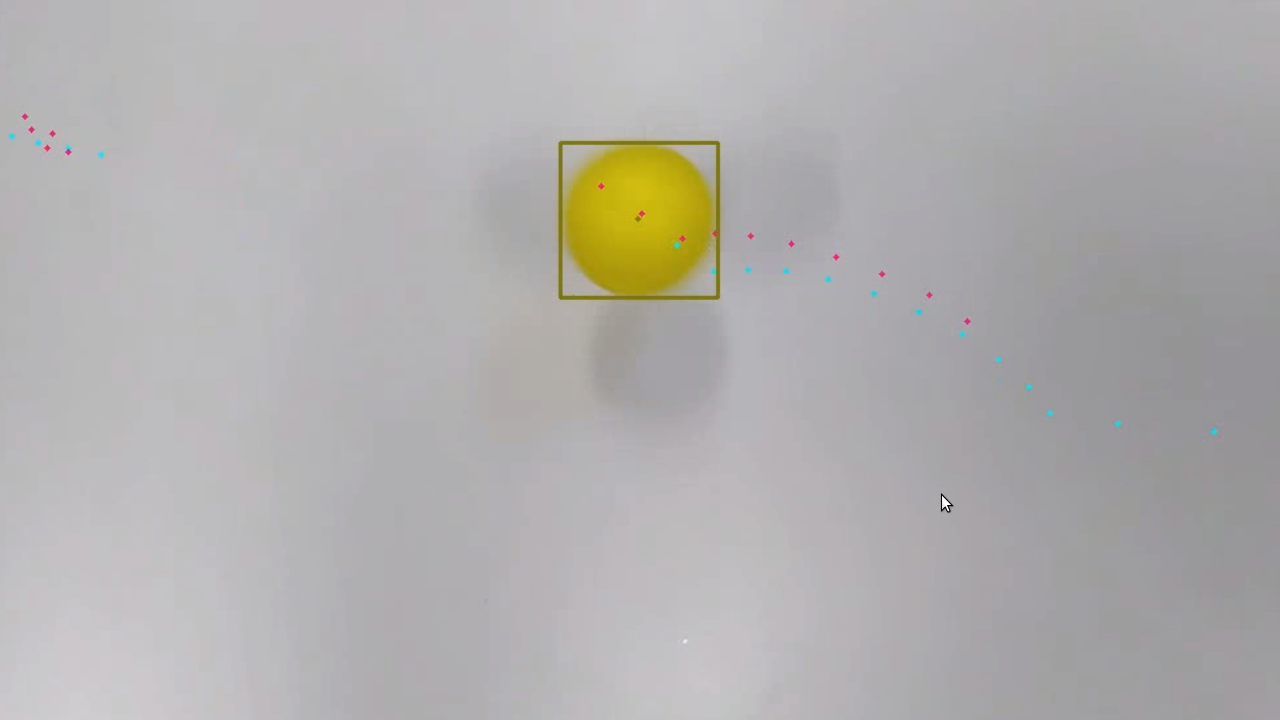
\includegraphics[scale=0.5]{images/motion}}
	\caption{Trajectory of the motion flow (pink) compared to the ball detection (light blue) on a bouncing ball.}
	\label{fig:motion}
\end{figure}

\textbf{Limitations of the Motion Flow and Hough Transform}:

\begin{figure}[!h]
	\centering
			\setlength{\fboxsep}{1pt}
			\setlength{\fboxrule}{1pt}
			\fbox{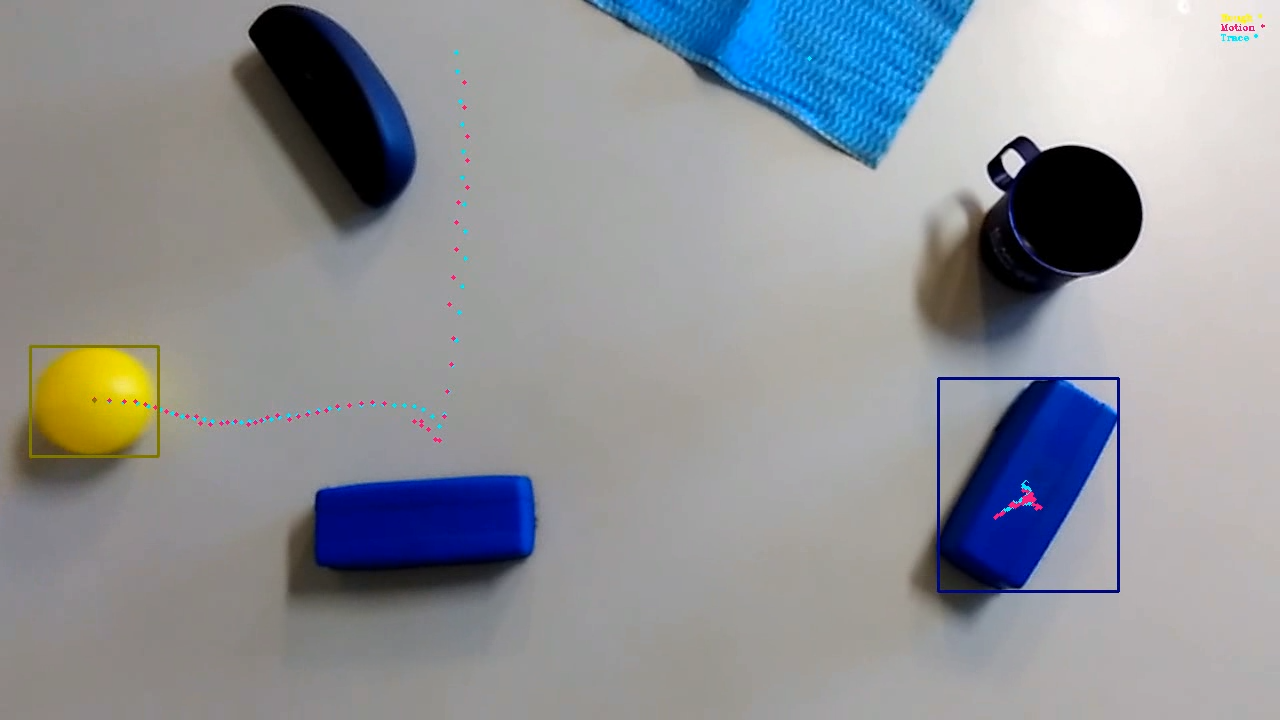
\includegraphics[scale=0.5]{images/motion_5}}
	\caption{Motion flow with an interval of 5 frames between resamples.}
	\label{fig:motion_10}
\end{figure}

\begin{figure}[!h]
	\centering
			\setlength{\fboxsep}{1pt}
			\setlength{\fboxrule}{1pt}
			\fbox{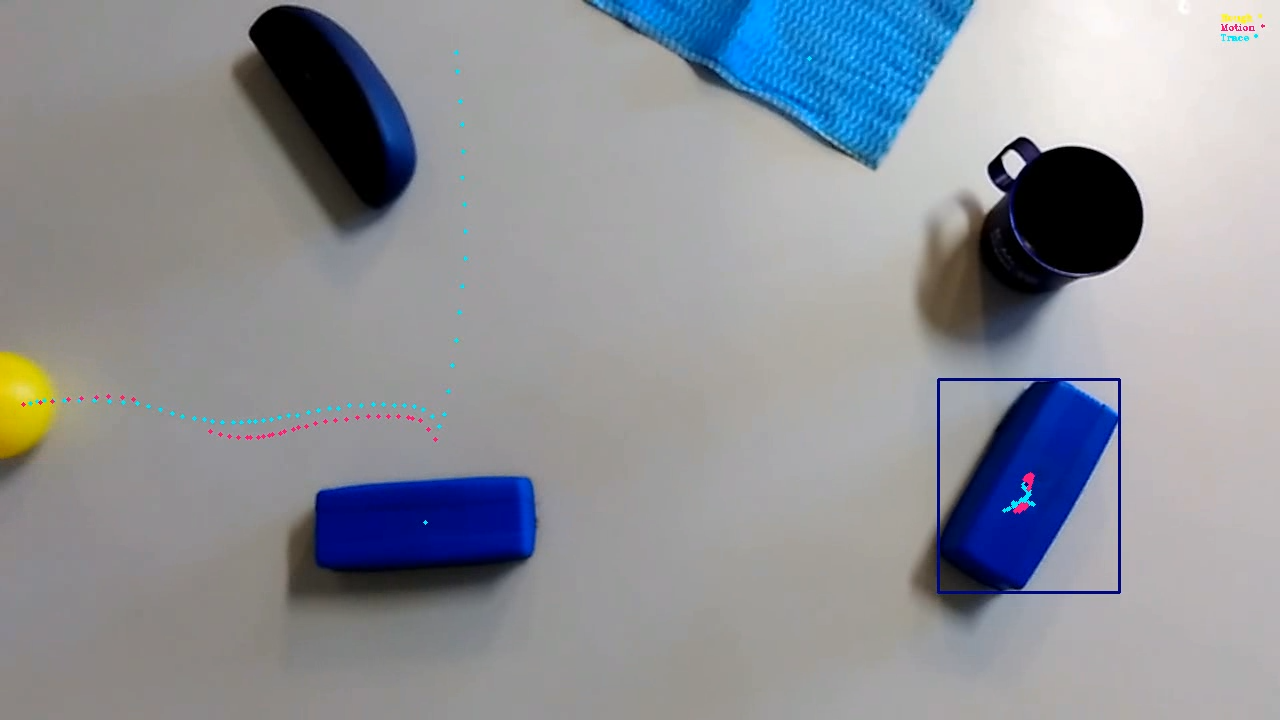
\includegraphics[scale=0.5]{images/motion_30}}
	\caption{Motion flow with an interval of 30 frames between resamples.}
	\label{fig:motion_50}
\end{figure}

\textbf{Kalman Filter Occlusion}:

\begin{figure}[!h]
	\centering
			\setlength{\fboxsep}{1pt}
			\setlength{\fboxrule}{1pt}
			\fbox{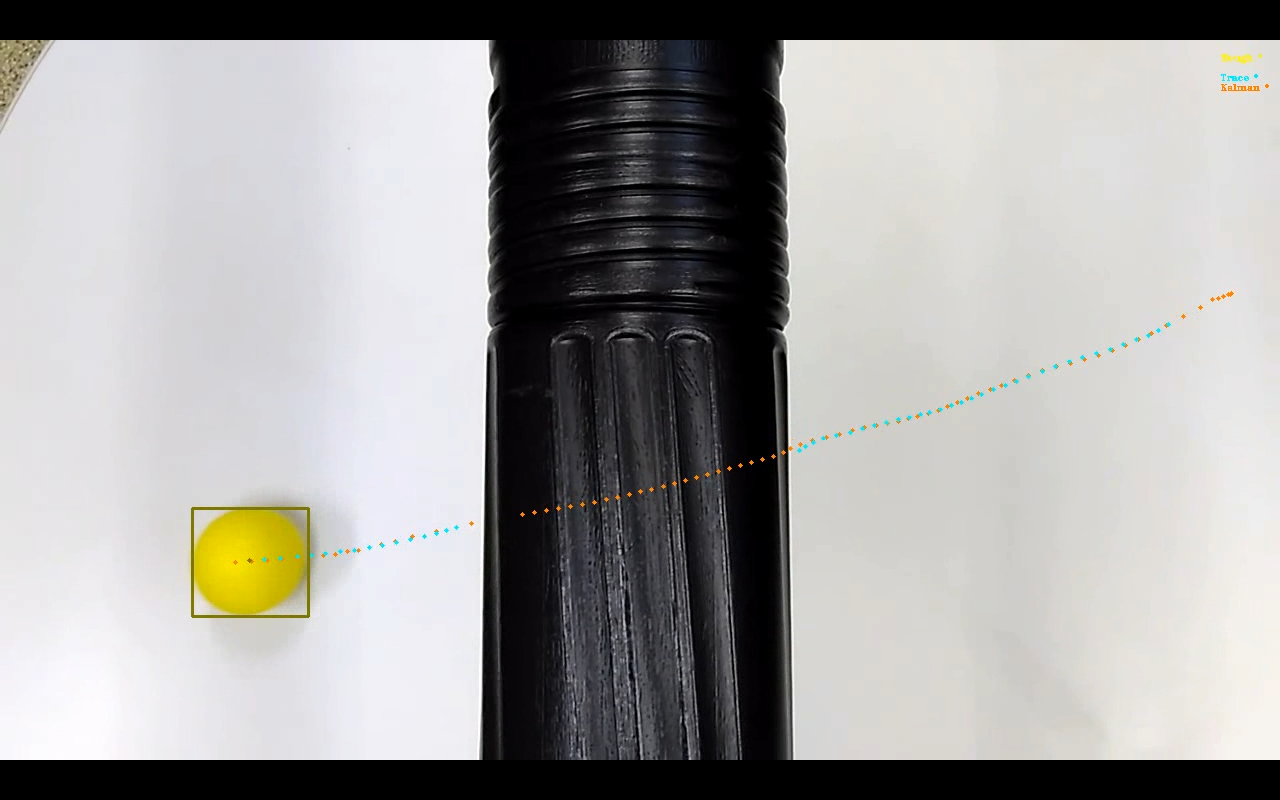
\includegraphics[scale=0.5]{images/occlusion}}
	\caption{Kalman filter (orange) predicting an occluded trajectory.}
	\label{fig:occlusion}
\end{figure}

\textbf{Real world application}:

\begin{figure}[!h]
	\centering
			\setlength{\fboxsep}{1pt}
			\setlength{\fboxrule}{1pt}
			\fbox{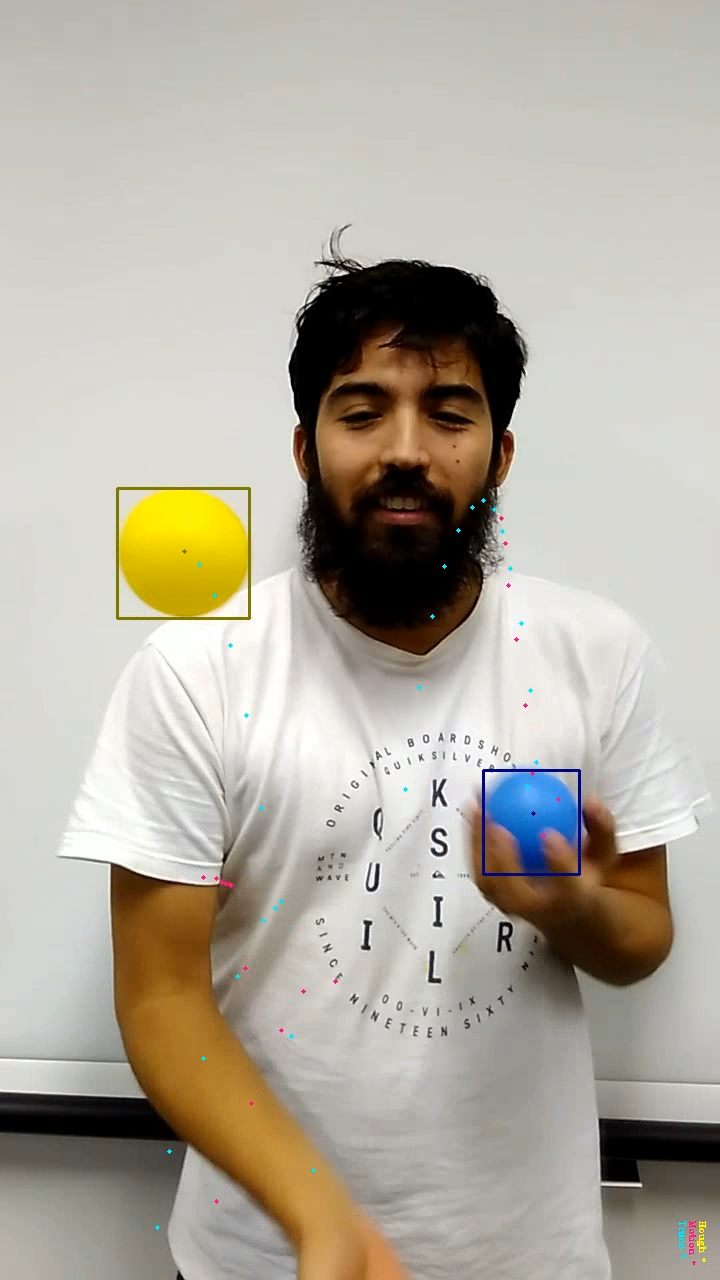
\includegraphics[scale=0.5]{images/miguel_1}}
	\caption{All implemented features working together to track the colored balls in a noisy background.}
	\label{fig:miguel_1}
\end{figure}

\begin{figure}[!h]
	\centering
			\setlength{\fboxsep}{1pt}
			\setlength{\fboxrule}{1pt}
			\fbox{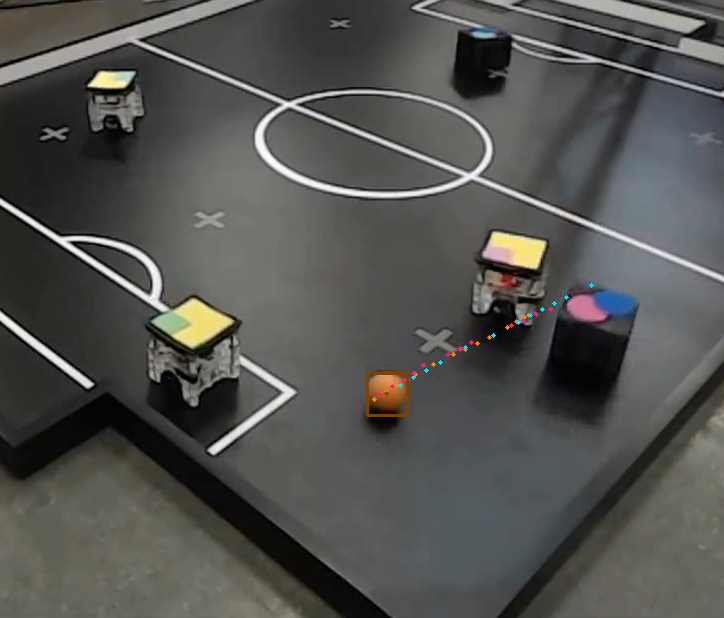
\includegraphics[scale=0.5]{images/robocup_1}}
	\caption{All implemented features working together to track a soccer match at Robo-cup.}
	\label{fig:robocup_1}
\end{figure}

\section{Conclusions}

The classic methods can present good results in a controlled environment, however it might have some difficulties in a noisy scenario as the real world. To perform in those complex scenarios, different set of tools are used in the literature, from physics model to deep neural networks.

\end{multicols}

\end{document}